% !TeX encoding = UTF-8
% !BIB program = biber
% DELFI 2026 – Designed but Not Used? A Feature Adoption Analysis of LiaScript Courses
%
% Build (im build/ Verzeichnis):
%   pdflatex main && biber main && pdflatex main && pdflatex main

\documentclass[biblatex, english]{lni}

\usepackage{booktabs}
\usepackage{multirow}
\usepackage{siunitx}
\sisetup{group-separator={.}, group-minimum-digits=4}
\usepackage{xcolor}
\usepackage{pgfplots}
\pgfplotsset{compat=1.18}

% TIKZ
\usepackage{tikz}
\usetikzlibrary{arrows.meta, positioning, fit, backgrounds, calc}

%% Farben für Feature-Kategorien
\definecolor{catPresentation}{HTML}{4393c3}
\definecolor{catInteraction}{HTML}{d6604d}
\definecolor{catReuse}{HTML}{4dac26}
\definecolor{catEmbedding}{HTML}{998ec3}

\addbibresource{../shared/literatur.bib}

\begin{document}

\title[LiaScript Feature Adoption]{Designed but Not Used? A Feature Adoption Analysis of LiaScript Courses}

\author[1]{Sebastian Zug}{sebastian.zug@informatik.tu-freiberg.de}{0000-0001-9949-6963}
\author[1]{André Dietrich}{andre.dietrich@informatik.tu-freiberg.de}{0000-0001-8894-1110}
\author[2]{Ines Aubel}{ines.aubel@chemie.tu-freiberg.de}{0000-0002-7589-9634}
\author[3]{Martin Lommatzsch}{m.lommatzsch@gsg-freiberg.lernsax.de}{?????}
\author[1]{Volker Göhler}{volker.goehler@informatik.tu-freiberg.de}{0000-0003-1901-1335}

\affil[1]{TU Bergakademie Freiberg\\Institut für Informatik\\09599 Freiberg\\Germany}
\affil[2]{TU Bergakademie Freiberg\\Institut für Technische Chemie\\09599 Freiberg\\Germany}
\affil[3]{Geschwister Scholl Gymnasium\\09599 Freiberg\\Germany}

\maketitle

\begin{abstract}

LiaScript is a Markdown-based language for creating interactive Open Educational Resources that runs entirely client-side, enabling courses to execute in the learner’s browser without server infrastructure. This sovereignty-by-design approach, due to eliminating accounts, server dependencies, and data-collection, gives educators full control over their content. However, this also eliminates the telemetry that would grant developers more insight into how pedagogical features are used in practice.

This paper addresses that gap through a corpus analysis of 3,317 validated LiaScript courses from public GitHub repositories (March 2026), contributed by 314 authors; of these, 2,973 courses with a clear education-level classification enter our group-level comparison. We introduce a didactically motivated taxonomy spanning presentation, interaction, reuse, and embedding features, and compare adoption across different authoring contexts --- core developers, a school-focused initiative, and independent community authors in higher education and school settings. Results show that 89\,\% of the designed feature space is adopted in measurable numbers, yet each community explores only its own subset: the challenge is not that features go unused, but that usage patterns vary strongly across contexts. Authoring infrastructure shapes adoption as strongly as pedagogical needs. We identify three adoption gap classes --- documentation deficits, workflow barriers, and configuration lock-in --- and derive context-sensitive implications for future development.
The study also demonstrates a replicable corpus methodology for understanding usage in OER that, by design, collects no user data.
\end{abstract}

\begin{keywords}
Open Educational Resources \and LiaScript \and Feature Adoption \and
OER Authoring \and Client-side Learning
\end{keywords}

\section{Introduction}
\label{sec:introduction}
% ~500 words
% Structure: OER challenge → LiaScript approach (with quiz example) →
%            blind spot → research questions

The creation of high-quality Open Educational Resources remains a persistent
challenge in higher education.
While content management systems and dedicated authoring tools exist,
they often impose significant technical barriers or proprietary lock-in,
discouraging educators from investing in interactive, reusable
materials~\cite{Henderson2018}.

\subsection{The LiaScript Approach}

LiaScript~\cite{Dietrich2019} takes a different approach: it extends standard
Markdown with interactive and multimedia elements using a human-readable syntax.
Listing~\ref{lst:quiz} illustrates this principle: a single-choice quiz
is expressed as a simple list with bracketed markers, directly within the
Markdown source.

\begin{figure}[ht]
  \begin{minipage}[t]{0.46\textwidth}
\begin{verbatim}
Where does DELFI 2026 take place?

- [( )] Munich
- [(X)] Potsdam
- [( )] Hamburg
[[?]] It is the capital of Brandenburg.
***
Potsdam hosts DELFI 2026 together
with HDI at the University of Potsdam.
***
\end{verbatim}
  \end{minipage}%
  \hfill
  \begin{minipage}[t]{0.50\textwidth}
    \vspace{0pt}
    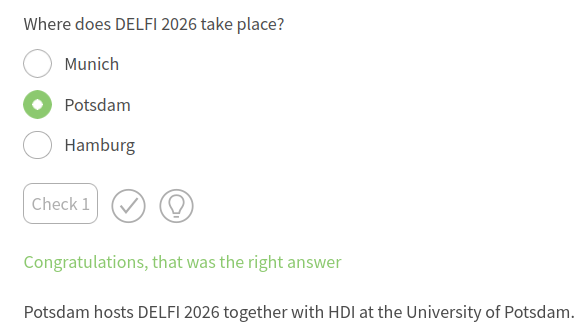
\includegraphics[width=\textwidth]{static_figures/Screenshot.png}
  \end{minipage}
  \caption{A LiaScript single-choice quiz: Markdown source (left) and
           rendered output (right).}
  \label{lst:quiz}
\end{figure}

Beyond quizzes, the language supports text-to-speech narration, animations,
executable code environments, reusable macro libraries, and many more
didactic elements --- all authored as plain text.
Unlike H5P, which requires a server and a Moodle/WordPress installation,
or Jupyter Book,
LiaScript executes without backend infrastructure.
A course file is a standard \texttt{.md} file; the LiaScript interpreter
is loaded client-side via a single URL.
An author pushes the file to any public Git host
and shares a link of the form \texttt{https://liascript.github.io/course/?URL}.
The browser fetches the file and interprets it locally;
no data is sent to any LiaScript server.

This client-side architecture is a deliberate design choice with significant
advantages: courses can be hosted anywhere, require no accounts, respect
learner privacy, and remain accessible even offline.
However, it introduces a fundamental blind spot for the developers.
Because no requests pass through a central server, \emph{there is no telemetry}.
The developers cannot observe which features are used, which courses are
accessed, or whether the pedagogical affordances built into the language
are exploited in practice.

\subsection{Contribution and Research Questions}

The only observable proxy for actual usage is the set of publicly available
LiaScript courses on GitHub.
This paper exploits that proxy systematically.
We analyse a corpus of \num{3317} validated courses from \num{307} committers,
introducing a didactically motivated taxonomy of LiaScript features and mapping
actual adoption rates onto the designed feature space.
The result is the first empirical picture of how LiaScript is used in the wild.

A key methodological choice is the segmentation of the corpus into three
groups: the LiaScript core developers (Internal), a prolific school-focused
power user (MINT-the-GAP), and the broader community.
This separation prevents the highly atypical output of the first two groups
from distorting aggregate adoption statistics.

Concretely, we address three research questions:
\begin{description}
  \item[RQ\,1] Which LiaScript features are adopted by the community and
               which remain underutilised?
  \item[RQ\,2] How do Internal, MINT-the-GAP, and Community groups differ
               in their feature adoption profiles?
  \item[RQ\,3] What development and documentation priorities follow from
               the identified adoption gaps?
\end{description}

The remainder of the paper is structured as follows.
Section~\ref{sec:background} reviews related work on OER tools, feature
adoption, and repository mining.
Section~\ref{sec:methodology} describes the feature taxonomy, the corpus,
and the three-group segmentation.
Section~\ref{sec:adoption} presents the empirical results.
Section~\ref{sec:implications} derives development priorities from the
identified adoption gaps, and
Section~\ref{sec:conclusion} summarises the contributions.


\section{Related Work}
\label{sec:background}
% Related Work – ca. 500 Wörter
% Drei Blöcke: OER-Tools, Feature-Adoption, GitHub-Mining

Analysing feature adoption in a client-side OER tool requires drawing on
three areas of prior work:
the \emph{OER authoring tool} landscape, which defines the design space
LiaScript operates in;
\emph{feature adoption research} in educational technologies, which
establishes that gaps between designed and used features are the norm
rather than the exception;
and \emph{repository mining}, which provides the methodological foundation
for studying a tool that produces no server-side telemetry.

\subsection{OER Authoring Tools}
\label{sec:rw:tools}

Several tools address the challenge of creating interactive educational content
from plain-text sources.
H5P~\cite{Kiryakova2022,Fornasari2025} is widely adopted for creating
self-contained interactive elements (quizzes, interactive videos) that can be
embedded in any LMS, but requires a server and does not support version control.
Jupyter Book~\cite{JupyterBook2025,Betlem2025} and mdBook generate complete
websites from Markdown files and integrate naturally with Git workflows, but
are primarily oriented towards computational and technical content.
The \emph{You Only Write Thrice} approach~\cite{WriteThrice2021} demonstrates
that a single Markdown source can generate a book, a slide deck, and a
computational notebook simultaneously --- a principle LiaScript generalises
to the full OER lifecycle.
Pandoc-based workflows~\cite{Krewinkel2017} address format interoperability
but do not add interactive pedagogical elements.
Git-based OER management has also been explored with GitLab as
infrastructure~\cite{Moser2025} and with GitHub specifically for
collaborative course development~\cite{Schwiertz2024}.

LiaScript differs from all of the above in combining Markdown simplicity,
rich interactive affordances, and a fully client-side execution model
that requires neither a server nor a pre-installed runtime~\cite{Baur2025}.

\subsection{Feature Adoption in Educational Technologies}
\label{sec:rw:adoption}

A recurring finding in educational technology research is that the number of
available features in a system far exceeds the number of features that are
actually used.
Studies on learning management systems document this pattern consistently:
Hijazi et al.~\cite{Hijazi2020} found a strong positive correlation between
feature \emph{awareness} and feature \emph{usage} in Moodle, with advanced
features such as SCORM packages and workshop modules remaining largely unknown
and therefore unused.
Awad et al.~\cite{Awad2019} observed similarly uneven utilisation of LMS
features even at well-resourced institutions.

The Technology Acceptance Model (TAM) and its extensions provide a theoretical
framework for these observations~\cite{Granic2022}.
Feng et al.~\cite{Feng2025} identify \emph{Effort Expectancy} --- the perceived
complexity of using a feature --- as the dominant predictor of non-adoption in
higher education contexts, outweighing perceived usefulness for features that
require significant authoring effort.

Crucially, all of these studies were conducted on server-based systems that
generate usage logs.
No prior work analyses feature adoption in a decentralised, client-side OER
tool where no telemetry is available and repository content is the only
observable proxy for usage behaviour.

\subsection{Mining Educational Repositories}
\label{sec:rw:mining}

Mining software repositories (MSR) is an established methodology for
understanding how tools are used in practice~\cite{Cosentino2017,Cosentino2016}.
Schröder and Pfänder~\cite{Schroeder2020} specifically explore GitHub as a
platform for OER, and Santos-Hermosa et al.~\cite{SantosHermosa2017} analyse
reuse indicators across OER repositories.
Both studies confirm that repository metadata --- commit history, contributor
counts, file content --- provides meaningful signals about authoring behaviour,
while also cautioning about the incompleteness of public repository data as a
usage proxy.

Our work extends this line of research by applying corpus analysis to a
specific OER authoring language, treating the GitHub corpus as the \emph{only
available substitute} for telemetry data in a privacy-preserving,
client-side tool.


\section{Dataset and Methodology}
\label{sec:methodology}
% ~600 words

\subsection{Data Collection Pipeline}

The dataset was constructed through a nine-stage pipeline
(\Cref{tab:data_pipeline} and \Cref{fig:data_pipeline_pub}), implemented in the open-source
\emph{ConnectedLecturer} project.\footnote{\url{https://github.com/TUBAF-IFI-ConnectedLecturer/Data_aggregation}}
Starting from GitHub's Search API, we identified \num{1076} repositories
containing potential LiaScript content.
A tree-level aggregation step extracted \num{57096} Markdown files,
of which \num{3317} (\SI{5.8}{\percent}) were validated as LiaScript courses
using a combination of rule-based filters and an LLM classifier
(Llama~3.3 70B).
For each course, the pipeline collected commit history (\num{19366} commits),
parsed header metadata (\SI{99.4}{\percent} success rate),
extracted \num{44} binary feature flags, and performed AI-based enrichment
(titles, keywords, educational level) for \SI{94.6}{\percent} of courses.
The final consolidated dataset comprises \num{3317} courses with
166~columns each (collected 2026-03-13).

%\begin{table}[ht]
%  \centering
%  \caption{Data collection pipeline stages}
%  \label{tab:pipeline}
%  \begin{tabular}{llr}
%    \toprule
%    \textbf{Phase} & \textbf{Method} & \textbf{$n$} \\
%    \midrule
%    Repository search    & GitHub Search API           & \num{1076} repos \\
%    File extraction      & Tree API + heuristics       & \num{57096} files \\
%    Validation           & Rules + LLM                 & \num{3317} courses (\SI{5.8}{\percent}) \\
%    Commit analysis      & Commits API                 & \num{19366} commits \\
%    Header metadata      & Regex parsing               & \num{3297} courses (\SI{99.4}{\percent}) \\
%    Feature detection    & 44 regex patterns            & $\num{3317} \times 44$ \\
%    AI enrichment        & RAG + Llama 3.3 70B         & \num{3138} courses (\SI{94.6}{\percent}) \\
%    User profiles        & GitHub Users API             & 445 profiles \\
%    Consolidation        & Inner join                   & $\num{3317} \times 166$ \\
%    \bottomrule
%  \end{tabular}
%\end{table}

\begin{table}[t]
\centering
\caption{Nine-stage data construction pipeline for the ConnectedLecturer dataset.}
\label{tab:data_pipeline}
\begin{tabular}{p{2.2cm} p{3.2cm} p{2.6cm} p{2.8cm}}
\toprule
\textbf{Phase} & \textbf{Method} & \textbf{Output} & \textbf{Coverage} \\
\midrule
Repository search 
& GitHub Search API 
& 1{,}076 repositories 
& -- \\

File extraction 
& Tree API + heuristics 
& 57{,}096 Markdown files 
& -- \\

Validation 
& Rule-based filters + LLM classifier 
& 3{,}317 LiaScript courses 
& 5.8\% of files \\

Commit analysis 
& Commits API 
& 19{,}366 commits 
& -- \\

Header metadata 
& Regex parsing 
& Metadata for 3{,}297 courses 
& 99.4\% of courses \\

Feature detection 
& 44 regex patterns 
& 44 features for 3{,}317 courses 
& 100\% \\

AI enrichment 
& RAG + Llama 3.3 70B 
& Enrichment for 3{,}138 courses 
& 94.6\% of courses \\

User profiles 
& GitHub Users API 
& 445 profiles 
& -- \\

Consolidation 
& Course-centered join 
& Final dataset: 3{,}317 courses $\times$ 166 columns 
& -- \\
\bottomrule
\end{tabular}
\end{table}

\begin{figure}[htbp]
\centering
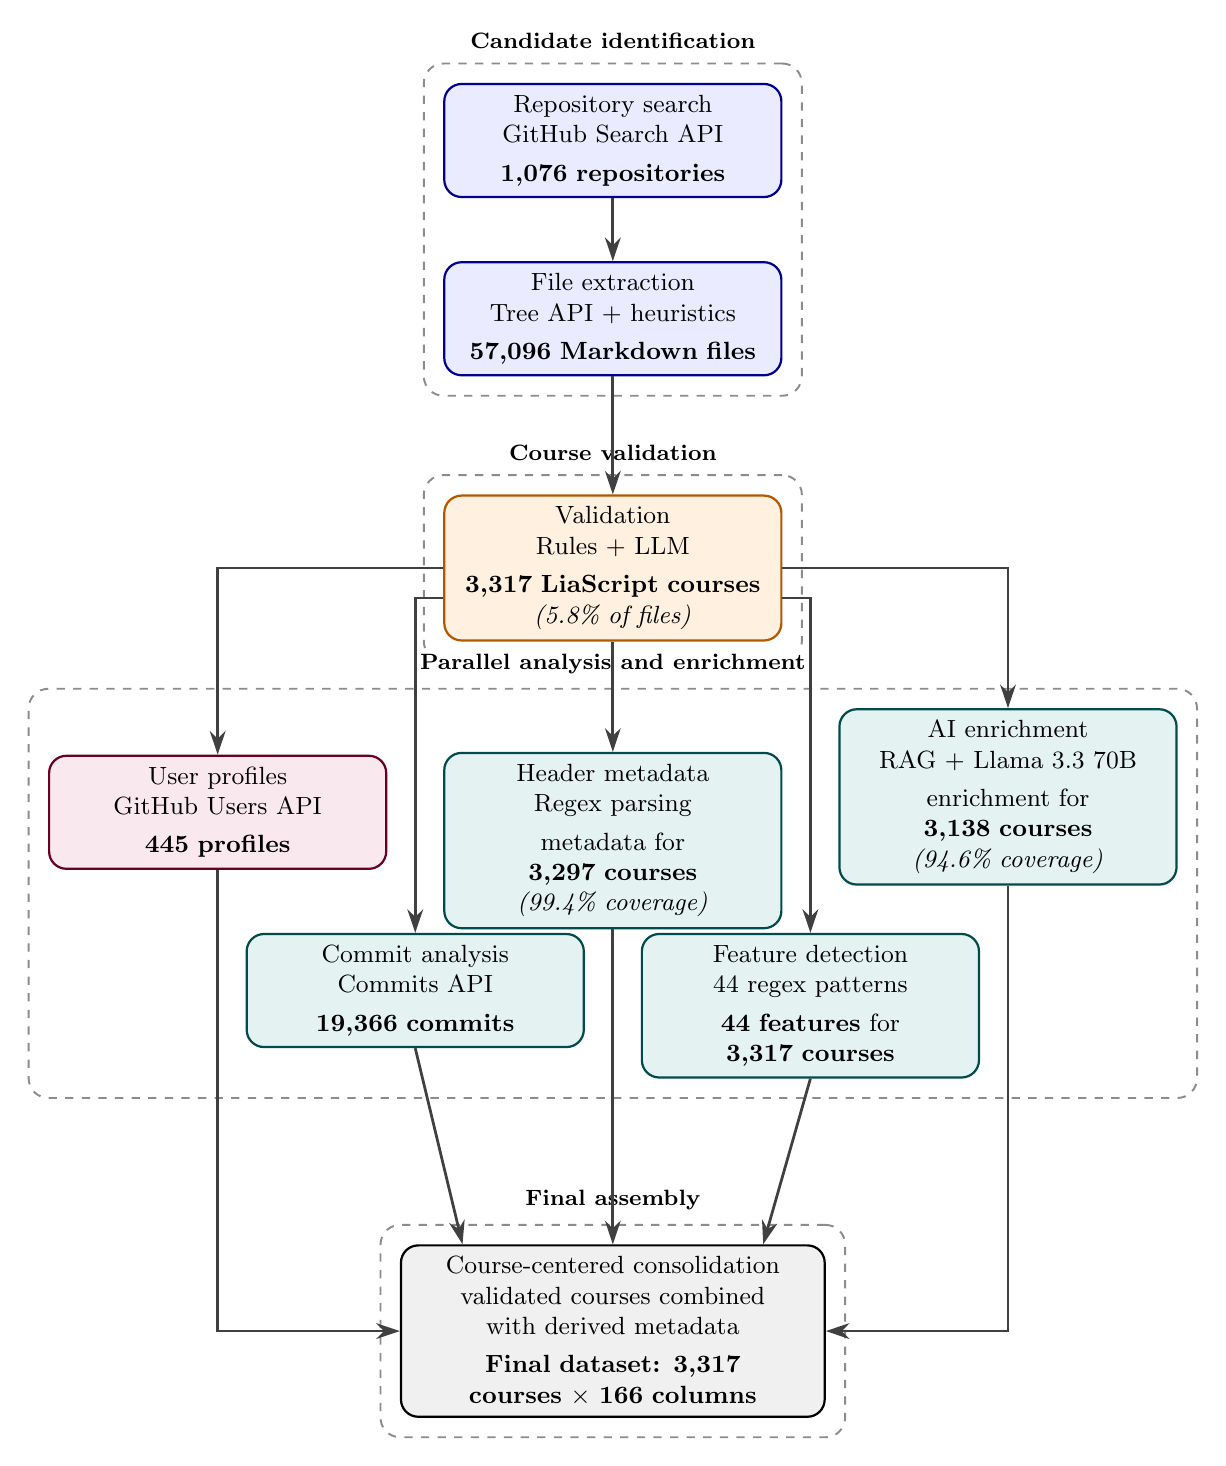
\begin{tikzpicture}[
    font=\small,
    node distance=8mm and 12mm,
    >={Stealth[length=3mm,width=2mm]},
    base/.style={
        rectangle,
        rounded corners=2.2mm,
        draw,
        line width=0.8pt,
        align=center,
        minimum height=1.35cm,
        text width=4.0cm,
        inner sep=4pt
    },
    search/.style={
        base,
        draw=blue!55!black,
        fill=blue!8
    },
    validate/.style={
        base,
        draw=orange!70!black,
        fill=orange!12
    },
    enrich/.style={
        base,
        draw=teal!60!black,
        fill=teal!10
    },
    aux/.style={
        base,
        draw=purple!55!black,
        fill=purple!9
    },
    finalbox/.style={
        base,
        draw=black,
        fill=gray!12,
        text width=5.1cm,
        minimum height=1.5cm
    },
    flow/.style={
        ->,
        line width=1.0pt,
        draw=black!75
    },
    groupbox/.style={
        rounded corners=2.5mm,
        draw=black!45,
        dashed,
        line width=0.7pt,
        inner sep=7pt
    },
    grouplabel/.style={
        font=\footnotesize\bfseries,
        fill=white,
        inner sep=2pt
    }
]

% --- Main linear path --------------------------------------------------------

\node[search] (search) {Repository search\\
GitHub Search API\\[1mm]
\textbf{1,076 repositories}};

\node[search, below=of search] (files) {File extraction\\
Tree API + heuristics\\[1mm]
\textbf{57,096 Markdown files}};

\node[validate, below=15mm of files] (valid) {Validation\\
Rules + LLM\\[1mm]
\textbf{3,317 LiaScript courses}\\
\emph{(5.8\% of files)}};

% --- Parallel branches -------------------------------------------------------

\node[enrich, below left=37mm and -18mm of valid] (commits) {Commit analysis\\
Commits API\\[1mm]
\textbf{19,366 commits}};

\node[enrich, below=14mm of valid] (header) {Header metadata\\
Regex parsing\\[1mm]
metadata for \textbf{3,297 courses}\\
\emph{(99.4\% coverage)}};

\node[enrich, below right=37mm and -18mm of valid] (features) {Feature detection\\
44 regex patterns\\[1mm]
\textbf{44 features} for\\
\textbf{3,317 courses}};

\node[enrich, above right= 6mm and -18mm of features] (ai) {AI enrichment\\
RAG + Llama 3.3 70B\\[1mm]
enrichment for \textbf{3,138 courses}\\
\emph{(94.6\% coverage)}};

\node[aux, above left= 8mm and -18mm of commits] (users) {User profiles\\
GitHub Users API\\[1mm]
\textbf{445 profiles}};

% --- Final node --------------------------------------------------------------

\node[finalbox, below=40mm of header] (final) {Course-centered consolidation\\
validated courses combined with derived metadata\\[1mm]
\textbf{Final dataset: 3,317 courses $\times$ 166 columns}};

% --- Arrows ------------------------------------------------------------------

\draw[flow] (search) -- (files);
\draw[flow] (files) -- (valid);

\draw[flow] (valid.190) -| (commits);
\draw[flow] (valid) -- (header);
\draw[flow] (valid.350) -| (features);
\draw[flow] (valid.east) -| (ai.north);
\draw[flow] (valid.west) -| (users.north);

\draw[flow] (users.south) |- (final.west);
\draw[flow] (commits.south) -- (final.150);
\draw[flow] (header) -- (final);
\draw[flow] (features.south) -- (final.30);
\draw[flow] (ai.south) |- (final.east);

% --- Group annotations -------------------------------------------------------

\begin{scope}[on background layer]
    \node[groupbox, fit=(search)(files)] (g1) {};
    \node[grouplabel, above=1mm of g1.north] {Candidate identification};

    \node[groupbox, fit=(valid)] (g2) {};
    \node[grouplabel, above=1mm of g2.north] {Course validation};

    \node[groupbox, fit=(users)(commits)(header)(features)(ai)] (g3) {};
    \node[grouplabel, above=1mm of g3.north] {Parallel analysis and enrichment};

    \node[groupbox, fit=(final)] (g4) {};
    \node[grouplabel, above=1mm of g4.north] {Final assembly};
\end{scope}

\end{tikzpicture}
\caption{Publication-oriented overview of the ConnectedLecturer data construction workflow. After candidate identification and course validation, several analysis and enrichment branches are executed in parallel and merged into the final consolidated course dataset.}
\label{fig:data_pipeline_pub}
\end{figure}

Our primary unit of analysis is the individual \emph{course file}
(one validated \texttt{.md} file = one course).
For grouping purposes courses are segmented by their \emph{repository
context} (Section~\ref{sec:three_groups}).

\subsection{Feature Taxonomy}
\label{sec:taxonomy}

For each course file the pipeline extracts \num{44} binary feature flags
via syntactic pattern matching on the Markdown source.\footnote{All regex patterns and their mapping to feature labels are documented at \url{https://github.com/TUBAF-IFI-ConnectedLecturer/Data_aggregation/blob/main/cl-pipeline/run/pipelines/liascript/docs/LiaScript_Features_Patterns.md}}
We organise these features into four didactically motivated categories
(Table~\ref{tab:taxonomy}).

\begin{table}[ht]
  \centering
  \caption{LiaScript feature taxonomy (4 categories, 44 tracked features)}
  \label{tab:taxonomy}
  \begin{tabular}{p{2.8cm}p{3.2cm}p{5.2cm}}
    \toprule
    \textbf{Category} & \textbf{Design intent} & \textbf{Representative features} \\
    \midrule
    \textcolor{catPresentation}{\textbf{Presentation}} &
      Self-paced, accessible delivery &
      Narrator (TTS), animations, effects, galleries \\[4pt]
    \textcolor{catInteraction}{\textbf{Interaction}} &
      Active learning \& formative feedback &
      Single/multiple choice, text input, matrix quiz, surveys \\[4pt]
    \textcolor{catReuse}{\textbf{Reuse}} &
      Scalable authoring via shared components &
      Imports, custom macros, official templates \\[4pt]
    \textcolor{catEmbedding}{\textbf{Embedding}} &
      Hands-on executable environments &
      Executable code, WebApps, external scripts, ASCII diagrams \\
    \bottomrule
  \end{tabular}
\end{table}

Each category addresses a different pedagogical barrier.
\emph{Presentation} features target accessibility (screen-reader-friendly TTS,
animated step-by-step reveals).
\emph{Interaction} features enable formative self-assessment without a learning
management system.
\emph{Reuse} features support the Don't-Repeat-Yourself principle at course level,
allowing shared building blocks across a curriculum.
\emph{Embedding} features close the gap between explanation and practice by
running code, simulations, or visualisations directly in the browser.

\subsection{Three-Group Segmentation}
\label{sec:three_groups}

Each course resides in a GitHub repository owned by an individual or
organisation account.
The \num{3317} courses were contributed by \num{307} unique committers
working across \num{205} repository accounts (\num{167}~individual,
\num{37}~organisational, 1~unclassified).
Organisation accounts act as hosting containers; the actual authors are
identified through the Git commit history (\texttt{contributors\_list}).

To prevent distortions from authors with fundamentally different
relationships to LiaScript, we segment courses into three groups based
on the \emph{repository context}:
\begin{description}
  \item[Internal] (462~courses, 7~repository accounts, 58~committers):
    Repositories owned by the core development team and their
    organisational accounts
    (SebastianZug, andre-dietrich, LiaPlayground, LiaScript, LiaBooks,
    LiaTemplates, TUBAF-IfI-LiaScript).
    These include templates, demonstrations, and the developers' own
    teaching materials.
  \item[MINT-the-GAP] (1\,147~courses, 1~organisation account, 3~committers):
    A single prolific school-focused initiative producing structured
    STEM courses.
    With nearly a third of all courses, this account would dominate any
    community-level analysis if not separated.
  \item[Community] (1\,708~courses, 197~repository accounts, 269~committers):
    All remaining courses, representing independent adoption by
    educators without direct involvement in LiaScript development.
    The group spans a wide range of engagement:
    82~accounts have produced exactly one course --- including
    test repositories, workshop materials, and one-off teaching
    projects --- while 8~accounts each contribute 56--146~courses.
    Despite this spread, no single account dominates
    (the largest accounts for \SI{8.5}{\percent}),
    and feature adoption rates show no systematic divergence between
    prolific and occasional contributors.
    Excluding all single-course accounts shifts adoption rates by
    less than one percentage point, confirming that the group is not
    distorted by test or tutorial content.
\end{description}

\noindent
Because grouping follows the repository context, the same committer
may appear in multiple groups.
In particular, 21~committers --- including the two core developers ---
contribute to both Internal and Community repositories.
Their work in Community repositories is counted as Community,
reflecting the collaborative context rather than the contributor's
identity.
For \num{306} courses (\SI{9.2}{\percent}) no commit history was
available; these are assigned solely based on their repository account.

\subsection{Complementary User Survey}
\label{sec:survey}

To triangulate the corpus findings, we conducted a structured needs
assessment with seven active LiaScript authors from different institutions
(March~2026).
Participants prioritised feature requests and usability issues on a
five-point scale.
The resulting 60~items are analysed qualitatively in
Section~\ref{sec:implications}.

\subsection{Limitations}

The corpus is restricted to \emph{public} GitHub repositories.
Courses hosted on other platforms, behind authentication, or in private
repositories are not captured.
Feature detection via pattern matching may miss features used through
indirect mechanisms (e.g.\ macros that generate quizzes programmatically).
The three-group segmentation assigns courses by repository context,
so the 21~committers active in multiple groups are counted in each
group separately rather than as a single entity.
The AI enrichment step (titles, keywords, DDC classification) was not
used in the present analysis but is available for future work.


\section{Feature Adoption in the Wild}
\label{sec:adoption}
Across the full corpus of \num{3317} courses, feature adoption varies
widely both between and within the four taxonomy categories.
Table~\ref{tab:adoption_overview} lists all tracked features sorted by
adoption rate within each category, revealing a clear gradient from
broadly adopted to virtually unused features.

\subsection{Aggregate Adoption Rates}

\begin{table}[ht]
  \centering
  \caption{Adoption rates across all \num{3317} courses, sorted by rate
           within each category.  Features above \SI{10}{\percent} are
           set in the left column, those below in the right.}
  \label{tab:adoption_overview}
  \begin{tabular}{@{}llr@{\qquad}lr@{}}
    \toprule
    & \multicolumn{2}{c}{\textbf{Widely adopted}} &
      \multicolumn{2}{c}{\textbf{Rarely adopted}} \\
    \textbf{Category} & \textbf{Feature} & \textbf{\%} &
      \textbf{Feature} & \textbf{\%} \\
    \midrule
    \multirow{4}{*}{\textcolor{catPresentation}{Presentation}}
      & Narrator        & 58.6 & Galleries      &  7.3 \\
      & Animations      & 22.8 & Animated CSS   &  0.7 \\
      & TTS fragments   & 11.6 & TTS blocks     &  0.1 \\
      & Anim.\ blocks   & 11.0 & Effects        &  0.0 \\
    \midrule
    \multirow{5}{*}{\textcolor{catInteraction}{Interaction}}
      & Any quiz        & 45.5 & Single choice  &  9.0 \\
      & Text quiz       & 28.8 & Quiz hints     &  4.9 \\
      & Multiple choice & 10.2 & Task lists     &  4.7 \\
      &                 &      & Surveys        &  2.7 \\
      &                 &      & Matrix quiz    &  1.6 \\
    \midrule
    \multirow{3}{*}{\textcolor{catReuse}{Reuse}}
      & Macros (any)    & 72.1 & Custom macros  &  8.7 \\
      & Imports         & 59.6 &                &      \\
      & Ext.\ scripts   & 51.1 &                &      \\
    \midrule
    \multirow{4}{*}{\textcolor{catEmbedding}{Embedding}}
      & Math            & 48.0 & ASCII diagrams &  9.8 \\
      & Script tags     & 20.8 & WebApps        &  5.6 \\
      & HTML embeds     & 15.7 & Exec.\ code    &  3.1 \\
      &                 &      & Code projects  &  0.4 \\
    \bottomrule
  \end{tabular}
\end{table}

The table reveals several patterns.
\textcolor{catPresentation}{Presentation} features split sharply: narrator
and animations require minimal authoring effort (a single comment line
activates TTS) and achieve broad uptake, while fine-grained variants
remain near zero.
\textcolor{catReuse}{Reuse} features are driven by the import and macro system
--- most authors \emph{consume} shared libraries and macros but few
\emph{define} custom macros (\SI{8.7}{\percent}).
\textcolor{catInteraction}{Interaction} is dominated by quizzes
(\SI{45.5}{\percent}), but survey and matrix quiz types remain rare.
\textcolor{catEmbedding}{Embedding} features show the widest internal
spread: math notation reaches \SI{48.0}{\percent} in STEM-oriented
courses, while executable code (\SI{3.1}{\percent}) and code projects
(\SI{0.4}{\percent}) remain niche despite being a signature LiaScript
capability.

\subsection{Group-level Adoption Profiles}
\label{sec:profiles}

Table~\ref{tab:group_diff} lists the features with notable adoption
differences across the three groups (spread $> 10$ percentage points).
Features with similar adoption rates across groups are omitted from the table
and discussed below.

\begin{table}[ht]
  \centering
  \caption{Features with divergent adoption rates across groups
           (spread $> 10$ pp).  The highest value per row is set in
           \textbf{bold}.}
  \label{tab:group_diff}
  \begin{tabular}{llrrr}
    \toprule
    \textbf{Category} & \textbf{Feature} &
      \textbf{Internal} & \textbf{MINT} & \textbf{Community} \\
    \midrule
    \multirow{5}{*}{\textcolor{catPresentation}{Presentation}}
      & Narrator       & \textbf{86.6} &  9.4 & 84.0 \\
      & TTS fragments  & \textbf{36.1} &  0.1 & 12.6 \\
      & Animations     & \textbf{66.2} &  0.6 & 25.9 \\
      & Anim.\ blocks  & \textbf{36.8} &  0.3 & 11.3 \\
      & Galleries      & \textbf{17.3} &  0.0 &  9.5 \\
    \midrule
    \multirow{4}{*}{\textcolor{catInteraction}{Interaction}}
      & Any quiz       & 22.7 & \textbf{78.3} & 29.6 \\
      & Single choice  & 11.9 &  0.2 & \textbf{14.1} \\
      & Multiple choice& 11.3 &  0.8 & \textbf{16.3} \\
      & Text quiz      &  9.7 & \textbf{70.0} &  6.2 \\
    \midrule
    \multirow{3}{*}{\textcolor{catReuse}{Reuse}}
      & Macros (any)   & 69.0 & \textbf{99.7} & 54.4 \\
      & Imports        & 57.4 & \textbf{98.3} & 34.3 \\
      & Ext.\ scripts  & 16.2 & \textbf{96.3} & 30.3 \\
    \midrule
    \multirow{5}{*}{\textcolor{catEmbedding}{Embedding}}
      & Exec.\ code    & \textbf{11.7} &  0.3 &  2.7 \\
      & WebApps        & \textbf{13.0} &  0.7 &  6.9 \\
      & Script tags    & \textbf{33.3} &  8.2 & 25.8 \\
      & ASCII diagrams & \textbf{38.5} &  2.3 &  7.1 \\
      & Math           & 30.7 & \textbf{95.2} & 21.0 \\
      & HTML embeds    & 18.6 &  5.9 & \textbf{21.5} \\
    \bottomrule
  \end{tabular}
\end{table}

Three patterns emerge from these divergences:

\paragraph{MINT-the-GAP's standardised configuration.}
MINT-the-GAP dominates the Reuse category (macros~\SI{99.7}{\percent},
imports~\SI{98.3}{\percent}, external scripts~\SI{96.3}{\percent})
and relies heavily on text quizzes (\SI{70.0}{\percent}) and
math notation (\SI{95.2}{\percent}).
This profile reflects a standardised configuration for small,
self-contained STEM exercises: each course file imports a common set
of libraries (TikZ visualisation, Algebrite CAS) and uses text quizzes
as the primary interactive element.
Notably, presentation features like narrator (\SI{9.4}{\percent}) and
animations (\SI{0.6}{\percent}) are nearly absent --- the exercise
format does not call for them.

\paragraph{Internal as feature showcase.}
The Internal group leads in presentation features (narrator~\SI{86.6}{\percent},
animations~\SI{66.2}{\percent}) and embedding features
(ASCII diagrams~\SI{38.5}{\percent}, script tags~\SI{33.3}{\percent}).
This is consistent with the developers' role as feature demonstrators and
early adopters of the full language surface.

\paragraph{Community as selective adopters.}
The Community group generally falls between the other two, but with
notable exceptions: single-choice (\SI{14.1}{\percent}) and
multiple-choice quizzes (\SI{16.3}{\percent}) are \emph{higher} than
in Internal, suggesting that community authors prefer familiar quiz
types over text-input quizzes.
HTML embeds (\SI{21.5}{\percent}) also peak in the Community group.

\paragraph{Convergent features.}
Several features show similar adoption across all three groups:
matrix quizzes (\SIrange{0.3}{2.4}{\percent}), surveys
(\SIrange{0.0}{4.8}{\percent}), task lists (\SIrange{0.0}{8.7}{\percent}),
and code projects (\SIrange{0.0}{1.3}{\percent}).
These consistently low rates indicate features that remain underutilised
regardless of author background, pointing to adoption barriers that
transcend group-specific workflows.


\section{Development Implications}
\label{sec:implications}
% ~750 words
% Five subsections: target audience, gap analysis, adoption ladder, survey, monitoring

The four-group comparison shows that prolific authors exhibit
the same feature profile as occasional contributors
(Section~\ref{sec:four_groups}) --- production volume does not drive
feature exploration.
Instead, the educational context shapes \emph{which} features authors
adopt: Comm-Uni authors gravitate toward narrated, code-heavy content;
Comm-School authors toward multimedia and interactive elements.
The MINT-the-GAP model demonstrates that infrastructure-level choices
can lift adoption for an entire community, but at the cost of narrowing
the explored feature space.
Effective improvements must therefore be \emph{context-sensitive}.

\subsection{Three Adoption Gap Classes}
\label{sec:gap_classes}

The adoption gradient itself can be explained through three gap classes.

\paragraph{Documentation deficit.}
Some features are syntactically non-obvious and lack progressive
examples.
Narrator adoption is high because activation requires a single header
line, whereas animation effects demand a multi-layered secondary syntax
documented only through a comprehensive reference.
The four-group comparison reinforces this: Comm-Uni authors show
significantly lower adoption of animation and script features than
Internal authors, while Comm-School authors --- despite lower narrator
adoption (\SI{60.8}{\percent} vs.\ \SI{88.5}{\percent}) --- achieve
higher rates of multimedia embedding.
The underlying syntax is identical, suggesting that documentation
does not sufficiently bridge the gap for either audience.

\paragraph{Workflow barrier.}
Code projects and executable code require authors to configure external
services and understand multi-file code block interactions ---
a barrier that documentation alone cannot resolve for non-technical
educators.

\paragraph{Configuration lock-in.}
The MINT-the-GAP profile demonstrates that a standardised configuration
--- importing the same libraries (TikZ, Algebrite) across all exercise
files --- can drive near-universal adoption of specific features
(math~\SI{95}{\percent}, imports~\SI{98}{\percent}), but simultaneously
leaves features outside this scope unexplored
(narrator~\SI{9}{\percent}, animations~\SI{0.6}{\percent}).
This pattern represents a design tension: standardised configurations
lower the entry barrier for a predefined feature set but discourage
exploration beyond it.
Future shared configurations should expose optional extension points
so that standardised workflows do not inadvertently narrow the
feature space.

Several features remain below \SI{5}{\percent} in \emph{all} four
groups, including among the core developers themselves
(animated CSS~\SI{2.4}{\percent}, code
projects~\SI{1.3}{\percent}, effects~\SI{0}{\percent}).
Unlike the documentation deficit, where Internal adoption proves that
the feature \emph{can} succeed, these convergent floors suggest that the
features' current design may not match real authoring needs.
They warrant a critical review of whether the feature concepts
themselves require rethinking rather than better documentation.

\subsection{The Adoption Ladder}
\label{sec:ladder}

The four-group analysis reveals that the adoption ladder differs
by educational context.
For \emph{Comm-Uni}, the progression runs:
narrator and links ($>$\,\SI{80}{\percent}) $\to$
code blocks, macros, and tables ($\approx$\,\SI{50}{\percent}) $\to$
animations and imports ($\approx$\,\SI{30}{\percent}) $\to$
embedding features ($<$\,\SI{10}{\percent}).
For \emph{Comm-School}, the ladder is structurally different:
links and images ($>$\,\SI{70}{\percent}) $\to$
macros, narrator, and logo ($\approx$\,\SI{55}{\percent}) $\to$
quizzes, imports, and multimedia ($\approx$\,\SI{35}{\percent}) $\to$
code and advanced embedding ($<$\,\SI{10}{\percent}).
The power-user analysis in Section~\ref{sec:four_groups} shows that
prolific authors exhibit essentially the same feature profile as
occasional contributors, indicating that production volume alone does
not drive feature exploration.
Onboarding documentation should therefore follow these ladders
explicitly and offer context-specific entry points for school vs.\
university authors.



\section{Conclusion}
\label{sec:conclusion}
% ~250 words

This paper presented the first systematic empirical analysis of feature
adoption in the LiaScript ecosystem.
Exploiting the GitHub corpus as the only observable proxy for a
tool with no server-side telemetry, we analysed \num{3317} courses
from \num{307} committers using a four-category feature taxonomy.

The central finding is a pronounced adoption gradient.
Presentation features --- particularly narrator/TTS and structural
animations --- are widely used, as is the macro and import system for
reuse.
Interactive affordances show selective adoption, while advanced embedding
features remain nearly invisible in practice despite being core
components of the LiaScript design.

This gradient mirrors a well-documented pattern in software engineering:
industry reports consistently find that roughly \SI{80}{\percent} of
features in software products are rarely or never used~\cite{pendo2019}.
Our three-group comparison adds nuance to this observation by showing
that different author communities exploit \emph{different} feature
subsets --- MINT-the-GAP's standardised configuration achieves
near-universal adoption of reuse and math features but leaves
presentation capabilities unexplored, while Community authors follow a natural
adoption ladder that plateaus well below the full feature space.
The HCI principle of \emph{progressive disclosure}~\cite{Nielsen2006}
--- revealing complexity only as users need it --- maps directly onto
this ladder and should guide future documentation design.
Notably, prolific authors show the same feature profile as occasional
contributors, indicating that experience alone does not drive
exploration --- a finding that underscores the need for \emph{active}
onboarding rather than relying on organic discovery.

These findings translate into three actionable priorities:
progressive documentation following the adoption ladder,
reduced embedding complexity through better tooling,
and shared configurations that expose rather than hide optional features.
AI-assisted course generation, identified as the top priority in a
complementary user survey, may address all three barriers simultaneously.

A companion study will shift the lens from feature adoption to course
\emph{lifecycle}: how courses evolve over time, how collaboration
manifests through commits and forks, and whether GitHub engagement
metrics (stars, forks) serve as valid indicators of educational impact
in a system that, by design, leaves no usage trace.


\printbibliography

\end{document}
